\subsection{Função Objetivo}

Composição da função objetivo:
\begin{itemize}
  \item KICK_POS_VARIATION
  \item WEIGHT_MOVE_DIST_TOTAL
  \item WEIGHT_MOVE_CHANGE
  \item WEIGHT_MOVE_DIST_MAX
  \item TOTAL_MAX_GAP_RATIO
% TOTAL_MAX_GAP_RATIO
% gap_value(){
%   return TOTAL_MAX_GAP_RATIO * total_gap + (1 - TOTAL_MAX_GAP_RATIO) * max_gap;
% }
  \item WEIGHT_ATTACK
  \item WEIGHT_SEE_ENEMY_GOAL
  \item WEIGHT_BLOCK_GOAL
  \item WEIGHT_BLOCK_ATTACKER
  \item WEIGHT_RECEIVERS_NUM
  \item DIST_GOAL_PENAL
  \item DIST_GOAL_TO_PENAL
\end{itemize}

Além dos parâmetros listados acima, outros parâmetros
afetam o comportamento do time:
\begin{itemize}
  \item MIN_GAP_TO_KICK
  \item RAMIFICATION_NUMBER
\end{itemize}

Esses parâmetros serão detalhados a seguir.

KICK_POS_VARIATION: o objetivo deste parâmetro é incorporar a monvimentação
do atacante no cálculo do \textit{gap} do gol. Isso pois defensores mais
próximos são mais facilmente driblados que defensores mais distantes. Isso
pode ser visualizado na figura \ref{fig:kick_pos_1}, onde foi considerada
uma variação de 15cm. Já na figura \ref{fig:kick_pos_2} foi considerada uma
variação de 0cm na posição da bola. Essa variação é medida na linha normal
à reta formada pela bola e pelo robô em questão.

\begin{figure}[h]
  \centering
  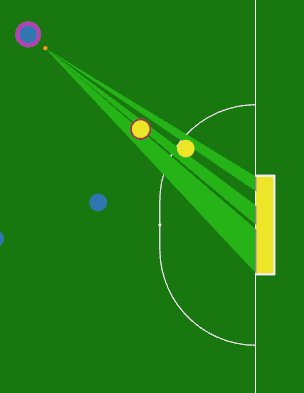
\includegraphics[width=0.8\linewidth]{kick_pos_var_1}
  \caption{\textit{Gap} do gol considerando-se uma variação de 15cm na 
           posição da bola}\label{fig:kick_pos_1}
  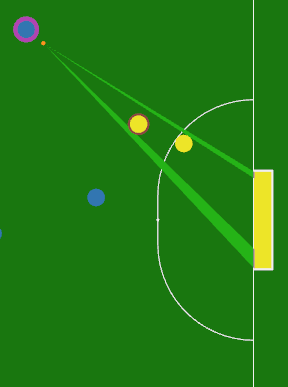
\includegraphics[width=0.8\linewidth]{kick_pos_var_2}
  \caption{\textit{Gap} do gol sem variação de na posição da
           bola}\label{fig:kick_pos_1}
\end{figure}


WEIGHT_MOVE_DIST_TOTAL: o objetivo deste parâmetro é incorporar o custo da
mudança de estado na função objetivo. Ele é formado pela soma dos \textit{
moves} de todos os robôs do time em questão.

WEIGHT_MOVE_DIST_MAX: o objetivo deste parâmetro é incorporar o custo da
mudança de estado na função objetivo. Ele é formado pelo \textit{move}
maior do planejamento atual.

WEIGHT_MOVE_CHANGE: o objetivo deste parâmetro é evitar mudanças grandes no
planejamento do move. Uma das razões para isso é evitar um mode dinâmico
exato neste nível de planejamento, já que isso aumentaria muito o custo
computacional desta etapa do planejamento e, consequentemente, reduziria
o número de simulações possíveis. Por essas razões mudanças no planejamento
dos \textit{moves} são penalizadas de acordo com a distância euclidiana
entre o \textit{move_p} planejado anteriormente e o \textit{move_m} modificado.
Isso permite que sejam selecionados \textit{moves_m} mais próximos do
\textit{move_p}, refinado assim o planejamento anterior.


TOTAL_MAX_GAP_RATIO: o objetivos deste parâmetro é valorizar \textit{gaps} maiores
de acordo com a soma total dos \textit{gaps} e com o maior \textit{gap}.
O cálculo do \textit{gap} é feito da seguinte maneira:

\begin{eqnarray} 
 gap value = TOTAL\_MAX\_GAP\_RATIO * \sum gap_i + (1 - TOTAL\_MAX\_GAP\_RATIO) * max{gap_i};
\end{eqnarray} 
